% article example for classicthesis.sty
\documentclass[10pt,a4paper]{article} % KOMA-Script article scrartcl
\usepackage{import}
\usepackage{xifthen}
\usepackage{pdfpages}
\usepackage{transparent}
\newcommand{\incfig}[1]{%
    \def\svgwidth{\columnwidth}
    \import{./figures/}{#1.pdf_tex}
}
\usepackage{lipsum}     %lorem ipsum text
\usepackage{titlesec}   %Section settings
\usepackage{titling}    %Title settings
\usepackage[margin=10em]{geometry}  %Adjusting margins
\usepackage{setspace}
\usepackage{listings}
\usepackage{amsmath}    %Display equations options
\usepackage{amssymb}    %More symbols
\usepackage{xcolor}     %Color settings
\usepackage{pagecolor}
\usepackage{mdframed}
\usepackage[spanish]{babel}
\usepackage[utf8]{inputenc}
\usepackage{longtable}
\usepackage{multicol}
\usepackage{graphicx}
\graphicspath{ {./Images/} }
\setlength{\columnsep}{1cm}

% ====| color de la pagina y del fondo |==== %
\pagecolor{white}
\color{black}



\begin{document}
    %========================{TITLE}====================%
    \title{\rmfamily\normalfont\spacedallcaps{ Tarea primera monitoría algebra abstracta }}
    \author{\spacedlowsmallcaps{Rodrigo Castillo}}
    \date{\today}

    \maketitle


     % ====| Loguito |==== %
    %=======================NOTES GOES HERE===================%
    \section{Principio de inducción fuerte:}
        \subsection{Demostración:}
            Sea $ S  $  el conjunto de todos los números naturales $ n  $  con
            que cumplen que
            que la propiedad  $ P(m)  $  se cumple en todos los m menores que m
            ($ m < n  $)
            .  Ahora, por inducción sobre $ n  $ tenemos que si $ n \in S  $
            entonces $ P(m)  $  se cumple para todo $ m < n  $
            \\ por hipotesis de induccion tenemos que $ P(n)  $ es verdadero.
            por lo tanto, cualquier numero $ m < n+1  $ también cumple la propiedad .
            \\ por lo tanto $ n +1 \in S  $
    \section{si n es un natural que no es un cuadrado perfecto entonces $ \sqrt{n}  $   es irracional.}
        sea $ n  $  un natural que no es un cuadrado perfecto , luego no existe
        $ m \in Z  $ tal que $ n = m ^{2}   $   .
        \\ supongamos que $ \sqrt{n}   $ es racional, por lo tanto existen $
        a,b \in Z  $ tales que $ \sqrt{n} = \frac{a}{b}   $ tales que $ a,b  $ son coprimos y $ mcd(a,b) = 1
        $
        \\ por lo tanto $ \frac{1}{n} = \frac{a ^{2 } }{b ^{2} }  $
        \\Ahora veamos que $ a ^{2}   $ y $ b ^{2}   $  también son coprimos ,
        por lo que por el teorema fundamental de la aritmetica y como
        consecuencia del lema de euclides, si existiera un primo que dividiera
        a $ a  $ y a $ b  $ entonces también dividiría a $ a ^{2}   $ y a $ b
        ^{2}   $   , pero supusimos que $ a ^{2}   $ y $ b ^{2}   $ eran
        coprimos, por lo que es una contradicción .

    \section{Utilice la fórmula de multiplicación entre números complejos en
    forma polar para encontrar los cuatros números complejos  que satisfacen $x ^{4}= 1   $ }
    dibujo para entender un poco :
    \\
        \begin{figure}[h]
            \centering
            \incfig{dibujo}
            \caption{dibujo}
        \end{figure}

        note que en la forma polar es mas fácil de ver la multiplicación de
        complejos, pues se suman sus angulos y se multiplican sus radios.

        \\ por lo tanto se tiene que :
        \begin{equation}
            r ^{4} = 1
        \end{equation}

        \begin{equation}
            ( \cos{\theta } \sin{\theta }) ^{4}  = 1
        \end{equation}

        \begin{equation}
            \theta  = \frac{n \pi }{2}
        \end{equation}

        \subsection{solución}

            de la ecuacion $ \theta  = \frac{n \pi }{2}  $ se obtienen 4 soluciones  , cuando
            \\ $ n = 0  $
            \\ $ n  = 1  $
            \\ $ n  = 2  $
            \\ $ n  =  3  $
            \\

            de los cuales se obtiene que $ theta = 0 , \frac{\pi }{2} , \pi  , \frac{3 \pi }{2}  $
            \\ por lo que las 4 soluciones son $ 1, i, -1 , -i  $

    \section{Demuestre que un polinomio a coeficientes reales de grado 2 o 3 es
    irreducible si y solo si no tiene ceros}

   $  \implies  $

        contrarreciprocra

        \\
        sea $ x  $  un polinomio de grado $ 2  $  o $ 3  $  reducible, por lo que
        existen 2 polinomios b,c tales que tales que $ b \times c   = x $ ,
        también sabemos que uno de los dos polinomios $ b   $ o $ c  $ es de
        grado 1  .
        \\ sea b el polinomio de grado 1 , por el teorema del residuo sabemos
        que es de la forma $ a - k  $ y y que la ecuacion $ a -k = 0  $ tiene
        solución, por lo tanto, $ k   $ es diferente de $ 0  $

        $ \Leftarrow  $
        sea $ x  $  un polinomio de grado 2 o 3 que tiene ceros , por lo tanto es
        de la forma $ x ^{2} + c   $  o $ x ^{3}  + c  $ luego existe $ x -c  $
        tales que $ F(x-c) = 0  $ , por lo tanto los polinomios son reducibles

    \section{Demuestre directamente que $ x ^{n} - c ^{n}   $  es divisible por
    x - c  para cualquier natural $ n  $ . Deduzca de esto el teorema del residuo visto en clase.}

        esto por el teorema del residuo es trivial, sin embargo, en internet
        encontré esta formula :
        \\ 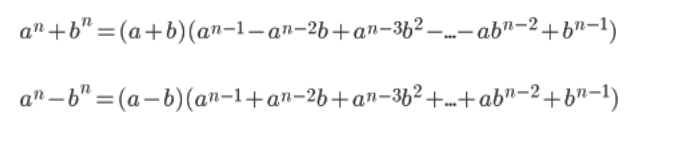
\includegraphics[width=0.8\linewidth]{internet.png}
        \\ acá ver que es divisible por $ x - c  $ es fácil, pues, sea $ k = (a
        ^{n-1} - a ^{n-2}b  + ... + b ^{n-2}a +... + b ^{n-1}    )  $ se tiene
        que existe $ k  $ tal que $ (x-c)k  $ = $ x ^{n} - c ^{n}   $

        \\ ahora deducir el teorema del reciduo basta con dividir toda la
        expresión sobre $ x-c  $ , por lo que quedaría que $ \frac{x ^{n} - c ^{n}  }{x-c} = \frac{x-c(k)}{x-c}   $
        y esa ecuación solamente tiene sentido cuando $ F(x-c)  = 0  $
        \section{sea $ m > 2  $  un entero , demuestre que hay m clases de
        equivalencia por la relacion ser congruente módulo $ m  $  y que son
        exactamente las clases $ [0] , [ 1] , ... , [m-1]  $ }

            induccion:
            \subsection{caso base}

                sea $ m = 2  $ , luego existe la clase de equivalencia $ [1] , [2]
                $ , sabemos que no existen mas clases de equivalencia pues suponer
                que existen mas clases de equivalencias es suponer que existe un
                número que es par e impar a la vez.

            \subsection{Caso inductivo}

                supongamos que para todo conjunto $ {0,1,2,3,4,5,6 ... n} $ en los
                enteros se cumple que existen  exactamente $ [0] , [1] , [2] , ..., [m-1]  $
                relaciones de equivalencia modulo $ m  $ , por lo que  $ m \mid
                (n-k)  $  , note que por propiedades de la división, $ m  $ no
                divide a $ (n+1) -k  $  , por lo que en el conjunto $ {0,1,2,3
                , 4, ...  , n+1}  $ existen las clases de equivalencia $ [0] ,
                [1] , ... , [m]  $  , luego existen exactamente m clases de equivalencia.


                \\
        \section{aviso}
        (soy consciente de que las demostraciones están super enredadas y
        en algunos casos mal elaboradas, sin embargo prometo practicar
        mas ejercicios de
        demostraciones  en el transcurso de esta semana)














    %=======================NOTES ENDS HERE===================%

    % bib stuff
    \nocite{*}
    \addtocontents{toc}{\protect\vspace{\beforebibskip}}

    \addcontentsline{toc}{section}{\refname}
    \bibliographystyle{plain}
    \bibliography{../Bibliography}
\end{document}
